\documentclass[]{article}
\usepackage{lmodern}
\usepackage{amssymb,amsmath}
\usepackage{ifxetex,ifluatex}
\usepackage{fixltx2e} % provides \textsubscript
\ifnum 0\ifxetex 1\fi\ifluatex 1\fi=0 % if pdftex
  \usepackage[T1]{fontenc}
  \usepackage[utf8]{inputenc}
\else % if luatex or xelatex
  \ifxetex
    \usepackage{mathspec}
  \else
    \usepackage{fontspec}
  \fi
  \defaultfontfeatures{Ligatures=TeX,Scale=MatchLowercase}
\fi
% use upquote if available, for straight quotes in verbatim environments
\IfFileExists{upquote.sty}{\usepackage{upquote}}{}
% use microtype if available
\IfFileExists{microtype.sty}{%
\usepackage{microtype}
\UseMicrotypeSet[protrusion]{basicmath} % disable protrusion for tt fonts
}{}
\usepackage[margin=1in]{geometry}
\usepackage{hyperref}
\hypersetup{unicode=true,
            pdftitle={DATA 606 - Lab 6},
            pdfborder={0 0 0},
            breaklinks=true}
\urlstyle{same}  % don't use monospace font for urls
\usepackage{color}
\usepackage{fancyvrb}
\newcommand{\VerbBar}{|}
\newcommand{\VERB}{\Verb[commandchars=\\\{\}]}
\DefineVerbatimEnvironment{Highlighting}{Verbatim}{commandchars=\\\{\}}
% Add ',fontsize=\small' for more characters per line
\usepackage{framed}
\definecolor{shadecolor}{RGB}{248,248,248}
\newenvironment{Shaded}{\begin{snugshade}}{\end{snugshade}}
\newcommand{\KeywordTok}[1]{\textcolor[rgb]{0.13,0.29,0.53}{\textbf{#1}}}
\newcommand{\DataTypeTok}[1]{\textcolor[rgb]{0.13,0.29,0.53}{#1}}
\newcommand{\DecValTok}[1]{\textcolor[rgb]{0.00,0.00,0.81}{#1}}
\newcommand{\BaseNTok}[1]{\textcolor[rgb]{0.00,0.00,0.81}{#1}}
\newcommand{\FloatTok}[1]{\textcolor[rgb]{0.00,0.00,0.81}{#1}}
\newcommand{\ConstantTok}[1]{\textcolor[rgb]{0.00,0.00,0.00}{#1}}
\newcommand{\CharTok}[1]{\textcolor[rgb]{0.31,0.60,0.02}{#1}}
\newcommand{\SpecialCharTok}[1]{\textcolor[rgb]{0.00,0.00,0.00}{#1}}
\newcommand{\StringTok}[1]{\textcolor[rgb]{0.31,0.60,0.02}{#1}}
\newcommand{\VerbatimStringTok}[1]{\textcolor[rgb]{0.31,0.60,0.02}{#1}}
\newcommand{\SpecialStringTok}[1]{\textcolor[rgb]{0.31,0.60,0.02}{#1}}
\newcommand{\ImportTok}[1]{#1}
\newcommand{\CommentTok}[1]{\textcolor[rgb]{0.56,0.35,0.01}{\textit{#1}}}
\newcommand{\DocumentationTok}[1]{\textcolor[rgb]{0.56,0.35,0.01}{\textbf{\textit{#1}}}}
\newcommand{\AnnotationTok}[1]{\textcolor[rgb]{0.56,0.35,0.01}{\textbf{\textit{#1}}}}
\newcommand{\CommentVarTok}[1]{\textcolor[rgb]{0.56,0.35,0.01}{\textbf{\textit{#1}}}}
\newcommand{\OtherTok}[1]{\textcolor[rgb]{0.56,0.35,0.01}{#1}}
\newcommand{\FunctionTok}[1]{\textcolor[rgb]{0.00,0.00,0.00}{#1}}
\newcommand{\VariableTok}[1]{\textcolor[rgb]{0.00,0.00,0.00}{#1}}
\newcommand{\ControlFlowTok}[1]{\textcolor[rgb]{0.13,0.29,0.53}{\textbf{#1}}}
\newcommand{\OperatorTok}[1]{\textcolor[rgb]{0.81,0.36,0.00}{\textbf{#1}}}
\newcommand{\BuiltInTok}[1]{#1}
\newcommand{\ExtensionTok}[1]{#1}
\newcommand{\PreprocessorTok}[1]{\textcolor[rgb]{0.56,0.35,0.01}{\textit{#1}}}
\newcommand{\AttributeTok}[1]{\textcolor[rgb]{0.77,0.63,0.00}{#1}}
\newcommand{\RegionMarkerTok}[1]{#1}
\newcommand{\InformationTok}[1]{\textcolor[rgb]{0.56,0.35,0.01}{\textbf{\textit{#1}}}}
\newcommand{\WarningTok}[1]{\textcolor[rgb]{0.56,0.35,0.01}{\textbf{\textit{#1}}}}
\newcommand{\AlertTok}[1]{\textcolor[rgb]{0.94,0.16,0.16}{#1}}
\newcommand{\ErrorTok}[1]{\textcolor[rgb]{0.64,0.00,0.00}{\textbf{#1}}}
\newcommand{\NormalTok}[1]{#1}
\usepackage{graphicx,grffile}
\makeatletter
\def\maxwidth{\ifdim\Gin@nat@width>\linewidth\linewidth\else\Gin@nat@width\fi}
\def\maxheight{\ifdim\Gin@nat@height>\textheight\textheight\else\Gin@nat@height\fi}
\makeatother
% Scale images if necessary, so that they will not overflow the page
% margins by default, and it is still possible to overwrite the defaults
% using explicit options in \includegraphics[width, height, ...]{}
\setkeys{Gin}{width=\maxwidth,height=\maxheight,keepaspectratio}
\IfFileExists{parskip.sty}{%
\usepackage{parskip}
}{% else
\setlength{\parindent}{0pt}
\setlength{\parskip}{6pt plus 2pt minus 1pt}
}
\setlength{\emergencystretch}{3em}  % prevent overfull lines
\providecommand{\tightlist}{%
  \setlength{\itemsep}{0pt}\setlength{\parskip}{0pt}}
\setcounter{secnumdepth}{0}
% Redefines (sub)paragraphs to behave more like sections
\ifx\paragraph\undefined\else
\let\oldparagraph\paragraph
\renewcommand{\paragraph}[1]{\oldparagraph{#1}\mbox{}}
\fi
\ifx\subparagraph\undefined\else
\let\oldsubparagraph\subparagraph
\renewcommand{\subparagraph}[1]{\oldsubparagraph{#1}\mbox{}}
\fi

%%% Use protect on footnotes to avoid problems with footnotes in titles
\let\rmarkdownfootnote\footnote%
\def\footnote{\protect\rmarkdownfootnote}

%%% Change title format to be more compact
\usepackage{titling}

% Create subtitle command for use in maketitle
\newcommand{\subtitle}[1]{
  \posttitle{
    \begin{center}\large#1\end{center}
    }
}

\setlength{\droptitle}{-2em}
  \title{DATA 606 - Lab 6}
  \pretitle{\vspace{\droptitle}\centering\huge}
  \posttitle{\par}
  \author{}
  \preauthor{}\postauthor{}
  \predate{\centering\large\emph}
  \postdate{\par}
  \date{11/12/2017}


\begin{document}
\maketitle

In August of 2012, news outlets ranging from the
\href{http://www.washingtonpost.com/national/on-faith/poll-shows-atheism-on-the-rise-in-the-us/2012/08/13/90020fd6-e57d-11e1-9739-eef99c5fb285_story.html}{Washington
Post} to the
\href{http://www.huffingtonpost.com/2012/08/14/atheism-rise-religiosity-decline-in-america_n_1777031.html}{Huffington
Post} ran a story about the rise of atheism in America. The source for
the story was a poll that asked people, ``Irrespective of whether you
attend a place of worship or not, would you say you are a religious
person, not a religious person or a convinced atheist?'' This type of
question, which asks people to classify themselves in one way or
another, is common in polling and generates categorical data. In this
lab we take a look at the atheism survey and explore what's at play when
making inference about population proportions using categorical data.

\subsection{The survey}\label{the-survey}

To access the press release for the poll, conducted by WIN-Gallup
International, click on the following link:

\emph{\url{http://www.wingia.com/web/files/richeditor/filemanager/Global_INDEX_of_Religiosity_and_Atheism_PR__6.pdf}}

Take a moment to review the report then address the following questions.

\subsection{Question 1}\label{question-1}

\begin{enumerate}
\def\labelenumi{\arabic{enumi}.}
\tightlist
\item
  In the first paragraph, several key findings are reported. Do these
  percentages appear to be \emph{sample statistics} (derived from the
  data sample) or \emph{population parameters}?
\end{enumerate}

\subsubsection{Solution}\label{solution}

Since we're using polling data, we're dealing with sample statistics.

\subsection{Question 2}\label{question-2}

\begin{enumerate}
\def\labelenumi{\arabic{enumi}.}
\setcounter{enumi}{1}
\tightlist
\item
  The title of the report is ``Global Index of Religiosity and
  Atheism''. To generalize the report's findings to the global human
  population, what must we assume about the sampling method? Does that
  seem like a reasonable assumption?
\end{enumerate}

\subsubsection{Solution}\label{solution-1}

The observations need to be independent, and we need the success-failure
condition (10 instances each of success and failure). Since these 50,000
samples comprise less than 10\% of the population, and the other two
conditions are satisfied, we can apply these inferences to the general
population.

\subsection{The data}\label{the-data}

Turn your attention to Table 6 (pages 15 and 16), which reports the
sample size and response percentages for all 57 countries. While this is
a useful format to summarize the data, we will base our analysis on the
original data set of individual responses to the survey. Load this data
set into R with the following command.

\begin{Shaded}
\begin{Highlighting}[]
\KeywordTok{load}\NormalTok{(}\StringTok{"more/atheism.RData"}\NormalTok{)}
\end{Highlighting}
\end{Shaded}

\subsection{Question 3}\label{question-3}

\begin{enumerate}
\def\labelenumi{\arabic{enumi}.}
\setcounter{enumi}{2}
\tightlist
\item
  What does each row of Table 6 correspond to? What does each row of
  \texttt{atheism} correspond to?
\end{enumerate}

\subsubsection{Solution}\label{solution-2}

Each row in table 6 is the cumulative survey results for that country.
Each row in \texttt{atheism} corresponds to an individual survey result.

To investigate the link between these two ways of organizing this data,
take a look at the estimated proportion of atheists in the United
States. Towards the bottom of Table 6, we see that this is 5\%. We
should be able to come to the same number using the \texttt{atheism}
data.

\subsection{Question 4}\label{question-4}

\begin{enumerate}
\def\labelenumi{\arabic{enumi}.}
\setcounter{enumi}{3}
\tightlist
\item
  Using the command below, create a new dataframe called \texttt{us12}
  that contains only the rows in \texttt{atheism} associated with
  respondents to the 2012 survey from the United States. Next, calculate
  the proportion of atheist responses. Does it agree with the percentage
  in Table 6? If not, why?
\end{enumerate}

\begin{Shaded}
\begin{Highlighting}[]
\NormalTok{us12 <-}\StringTok{ }\KeywordTok{subset}\NormalTok{(atheism, nationality }\OperatorTok{==}\StringTok{ "United States"} \OperatorTok{&}\StringTok{ }\NormalTok{year }\OperatorTok{==}\StringTok{ "2012"}\NormalTok{)}
\end{Highlighting}
\end{Shaded}

\subsubsection{Solution}\label{solution-3}

\begin{Shaded}
\begin{Highlighting}[]
\KeywordTok{sum}\NormalTok{(us12}\OperatorTok{$}\NormalTok{response }\OperatorTok{==}\StringTok{ "atheist"}\NormalTok{) }\OperatorTok{/}\StringTok{ }\KeywordTok{nrow}\NormalTok{(us12)}
\end{Highlighting}
\end{Shaded}

\begin{verbatim}
## [1] 0.0499002
\end{verbatim}

Yes, they both put the number of atheists in the US in 2012 at
\(\approx 5\%\).

\subsection{Inference on proportions}\label{inference-on-proportions}

As was hinted at in Exercise 1, Table 6 provides \emph{statistics}, that
is, calculations made from the sample of 51,927 people. What we'd like,
though, is insight into the population \emph{parameters}. You answer the
question, ``What proportion of people in your sample reported being
atheists?'' with a statistic; while the question ``What proportion of
people on earth would report being atheists'' is answered with an
estimate of the parameter.

The inferential tools for estimating population proportion are analogous
to those used for means in the last chapter: the confidence interval and
the hypothesis test.

\subsection{Question 5}\label{question-5}

\begin{enumerate}
\def\labelenumi{\arabic{enumi}.}
\setcounter{enumi}{4}
\tightlist
\item
  Write out the conditions for inference to construct a 95\% confidence
  interval for the proportion of atheists in the United States in 2012.
  Are you confident all conditions are met?
\end{enumerate}

\subsubsection{Solution}\label{solution-4}

The observations need to be independent, and a sufficiently large sample
size (success-failure condition). Since this sample is less than 10\% of
the US population, and there are at least 10 atheists and non-atheists,
both conditions have been satisfied.

If the conditions for inference are reasonable, we can either calculate
the standard error and construct the interval by hand, or allow the
\texttt{inference} function to do it for us.

\begin{Shaded}
\begin{Highlighting}[]
\KeywordTok{inference}\NormalTok{(us12}\OperatorTok{$}\NormalTok{response, }\DataTypeTok{est =} \StringTok{"proportion"}\NormalTok{, }\DataTypeTok{type =} \StringTok{"ci"}\NormalTok{, }\DataTypeTok{method =} \StringTok{"theoretical"}\NormalTok{, }
          \DataTypeTok{success =} \StringTok{"atheist"}\NormalTok{)}
\end{Highlighting}
\end{Shaded}

\begin{verbatim}
## Single proportion -- success: atheist 
## Summary statistics:
\end{verbatim}

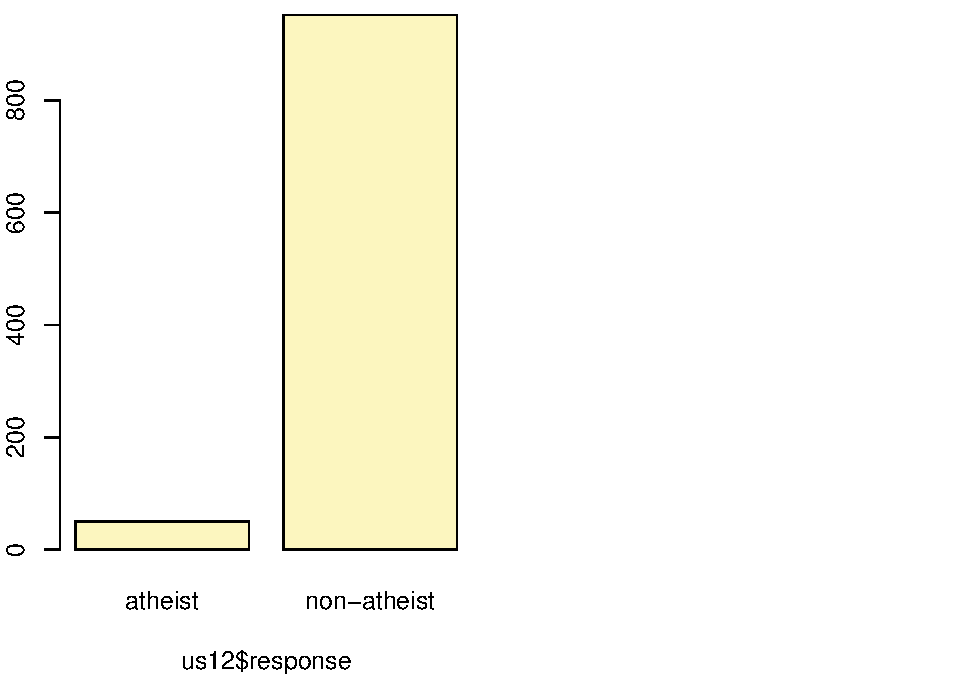
\includegraphics{DATA_606_Lab_6_files/figure-latex/us-atheism-ci-1.pdf}

\begin{verbatim}
## p_hat = 0.0499 ;  n = 1002 
## Check conditions: number of successes = 50 ; number of failures = 952 
## Standard error = 0.0069 
## 95 % Confidence interval = ( 0.0364 , 0.0634 )
\end{verbatim}

Note that since the goal is to construct an interval estimate for a
proportion, it's necessary to specify what constitutes a ``success'',
which here is a response of \texttt{"atheist"}.

Although formal confidence intervals and hypothesis tests don't show up
in the report, suggestions of inference appear at the bottom of page 7:
``In general, the error margin for surveys of this kind is \(\pm\) 3-5\%
at 95\% confidence''.

\subsection{Question 6}\label{question-6}

\begin{enumerate}
\def\labelenumi{\arabic{enumi}.}
\setcounter{enumi}{5}
\tightlist
\item
  Based on the R output, what is the margin of error for the estimate of
  the proportion of the proportion of atheists in US in 2012?
\end{enumerate}

\subsubsection{Solution}\label{solution-5}

\begin{Shaded}
\begin{Highlighting}[]
\NormalTok{(}\FloatTok{0.0634} \OperatorTok{-}\StringTok{ }\FloatTok{0.0364}\NormalTok{)}\OperatorTok{/}\DecValTok{2}
\end{Highlighting}
\end{Shaded}

\begin{verbatim}
## [1] 0.0135
\end{verbatim}

The margin of error is approximately 1.35\%.

\subsection{Question 7}\label{question-7}

\begin{enumerate}
\def\labelenumi{\arabic{enumi}.}
\setcounter{enumi}{6}
\tightlist
\item
  Using the \texttt{inference} function, calculate confidence intervals
  for the proportion of atheists in 2012 in two other countries of your
  choice, and report the associated margins of error. Be sure to note
  whether the conditions for inference are met. It may be helpful to
  create new data sets for each of the two countries first, and then use
  these data sets in the \texttt{inference} function to construct the
  confidence intervals.
\end{enumerate}

\subsection{Solution}\label{solution-6}

We'll compare Canada and the Netherlands.

\begin{Shaded}
\begin{Highlighting}[]
\NormalTok{ca12 <-}\StringTok{ }\KeywordTok{subset}\NormalTok{(atheism, nationality }\OperatorTok{==}\StringTok{ "Canada"} \OperatorTok{&}\StringTok{ }\NormalTok{year }\OperatorTok{==}\StringTok{ "2012"}\NormalTok{)}
\NormalTok{ca.prop <-}\StringTok{ }\KeywordTok{sum}\NormalTok{(ca12}\OperatorTok{$}\NormalTok{response }\OperatorTok{==}\StringTok{ "atheist"}\NormalTok{) }\OperatorTok{/}\StringTok{ }\KeywordTok{nrow}\NormalTok{(ca12)}
\NormalTok{ca.moe <-}\StringTok{ }\NormalTok{(}\FloatTok{0.1075} \OperatorTok{-}\StringTok{ }\FloatTok{0.0721}\NormalTok{) }\OperatorTok{/}\StringTok{ }\DecValTok{2}

\NormalTok{nl12 <-}\StringTok{ }\NormalTok{us12 <-}\StringTok{ }\KeywordTok{subset}\NormalTok{(atheism, nationality }\OperatorTok{==}\StringTok{ "Netherlands"} \OperatorTok{&}\StringTok{ }\NormalTok{year }\OperatorTok{==}\StringTok{ "2012"}\NormalTok{)}
\NormalTok{nl.prop <-}\StringTok{ }\KeywordTok{sum}\NormalTok{(nl12}\OperatorTok{$}\NormalTok{response }\OperatorTok{==}\StringTok{ "atheist"}\NormalTok{) }\OperatorTok{/}\StringTok{ }\KeywordTok{nrow}\NormalTok{(nl12)}
\NormalTok{nl.moe <-}\StringTok{ }\NormalTok{(}\FloatTok{0.1696} \OperatorTok{-}\StringTok{ }\FloatTok{0.1094}\NormalTok{) }\OperatorTok{/}\StringTok{ }\DecValTok{2}
  
\KeywordTok{inference}\NormalTok{(ca12}\OperatorTok{$}\NormalTok{response, }\DataTypeTok{est =} \StringTok{"proportion"}\NormalTok{, }\DataTypeTok{type =} \StringTok{"ci"}\NormalTok{, }\DataTypeTok{method =} \StringTok{"theoretical"}\NormalTok{, }
          \DataTypeTok{success =} \StringTok{"atheist"}\NormalTok{)}
\end{Highlighting}
\end{Shaded}

\begin{verbatim}
## Single proportion -- success: atheist 
## Summary statistics:
\end{verbatim}

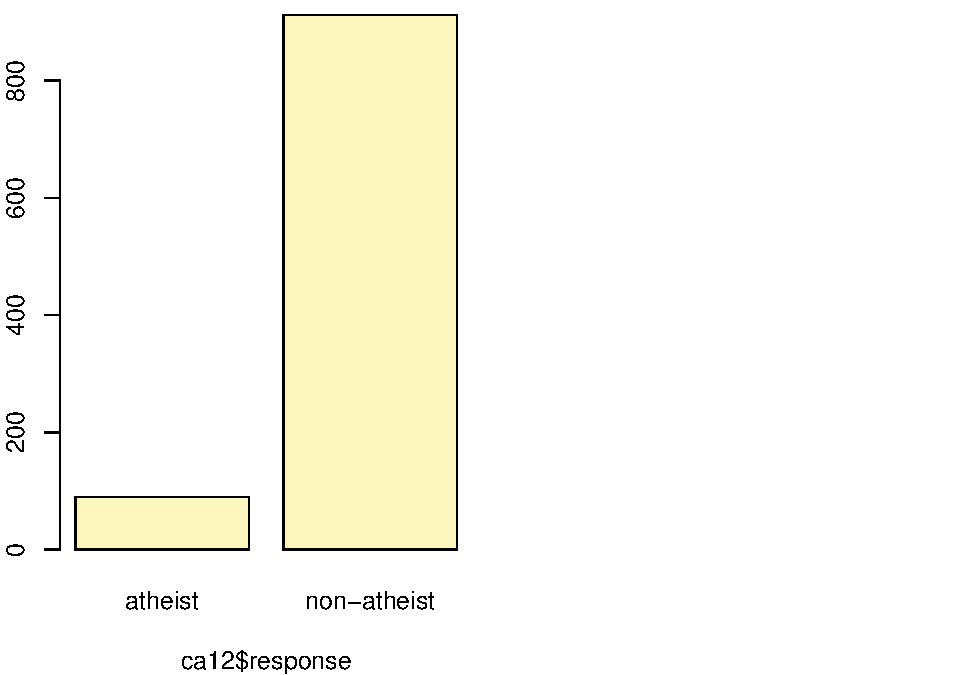
\includegraphics{DATA_606_Lab_6_files/figure-latex/unnamed-chunk-3-1.pdf}

\begin{verbatim}
## p_hat = 0.0898 ;  n = 1002 
## Check conditions: number of successes = 90 ; number of failures = 912 
## Standard error = 0.009 
## 95 % Confidence interval = ( 0.0721 , 0.1075 )
\end{verbatim}

\begin{Shaded}
\begin{Highlighting}[]
\KeywordTok{inference}\NormalTok{(nl12}\OperatorTok{$}\NormalTok{response, }\DataTypeTok{est =} \StringTok{"proportion"}\NormalTok{, }\DataTypeTok{type =} \StringTok{"ci"}\NormalTok{, }\DataTypeTok{method =} \StringTok{"theoretical"}\NormalTok{, }
          \DataTypeTok{success =} \StringTok{"atheist"}\NormalTok{)}
\end{Highlighting}
\end{Shaded}

\begin{verbatim}
## Single proportion -- success: atheist 
## Summary statistics:
\end{verbatim}

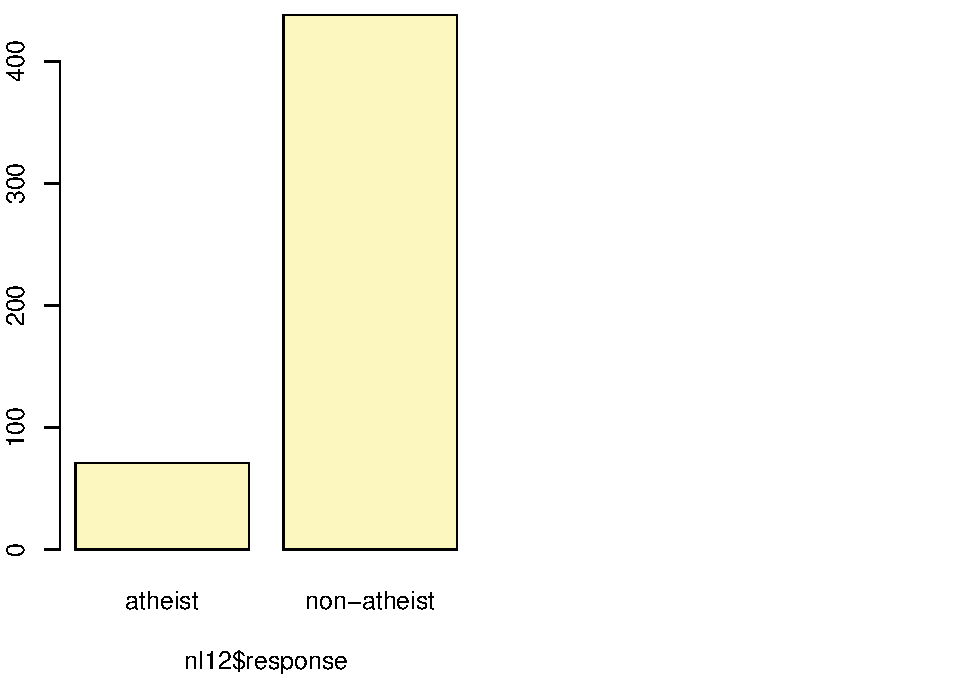
\includegraphics{DATA_606_Lab_6_files/figure-latex/unnamed-chunk-3-2.pdf}

\begin{verbatim}
## p_hat = 0.1395 ;  n = 509 
## Check conditions: number of successes = 71 ; number of failures = 438 
## Standard error = 0.0154 
## 95 % Confidence interval = ( 0.1094 , 0.1696 )
\end{verbatim}

In both cases, the sample size is less than 10\% of the country's
population, and there are at least 10 successes and 10 failures. The
margin of error for Canada is \(\approx 1.77\%\). The margin of error
for the Netherlands is \(\approx 3.01\%\).

\subsection{How does the proportion affect the margin of
error?}\label{how-does-the-proportion-affect-the-margin-of-error}

Imagine you've set out to survey 1000 people on two questions: are you
female? and are you left-handed? Since both of these sample proportions
were calculated from the same sample size, they should have the same
margin of error, right? Wrong! While the margin of error does change
with sample size, it is also affected by the proportion.

Think back to the formula for the standard error:
\(SE = \sqrt{p(1-p)/n}\). This is then used in the formula for the
margin of error for a 95\% confidence interval:
\(ME = 1.96\times SE = 1.96\times\sqrt{p(1-p)/n}\). Since the population
proportion \(p\) is in this \(ME\) formula, it should make sense that
the margin of error is in some way dependent on the population
proportion. We can visualize this relationship by creating a plot of
\(ME\) vs. \(p\).

The first step is to make a vector \texttt{p} that is a sequence from 0
to 1 with each number separated by 0.01. We can then create a vector of
the margin of error (\texttt{me}) associated with each of these values
of \texttt{p} using the familiar approximate formula
(\(ME = 2 \times SE\)). Lastly, we plot the two vectors against each
other to reveal their relationship.

\begin{Shaded}
\begin{Highlighting}[]
\NormalTok{n <-}\StringTok{ }\DecValTok{1000}
\NormalTok{p <-}\StringTok{ }\KeywordTok{seq}\NormalTok{(}\DecValTok{0}\NormalTok{, }\DecValTok{1}\NormalTok{, }\FloatTok{0.01}\NormalTok{)}
\NormalTok{moe <-}\StringTok{ }\DecValTok{2} \OperatorTok{*}\StringTok{ }\KeywordTok{sqrt}\NormalTok{(p }\OperatorTok{*}\StringTok{ }\NormalTok{(}\DecValTok{1} \OperatorTok{-}\StringTok{ }\NormalTok{p)}\OperatorTok{/}\NormalTok{n)}
\KeywordTok{plot}\NormalTok{(moe }\OperatorTok{~}\StringTok{ }\NormalTok{p, }\DataTypeTok{ylab =} \StringTok{"Margin of Error"}\NormalTok{, }\DataTypeTok{xlab =} \StringTok{"Population Proportion"}\NormalTok{)}
\end{Highlighting}
\end{Shaded}

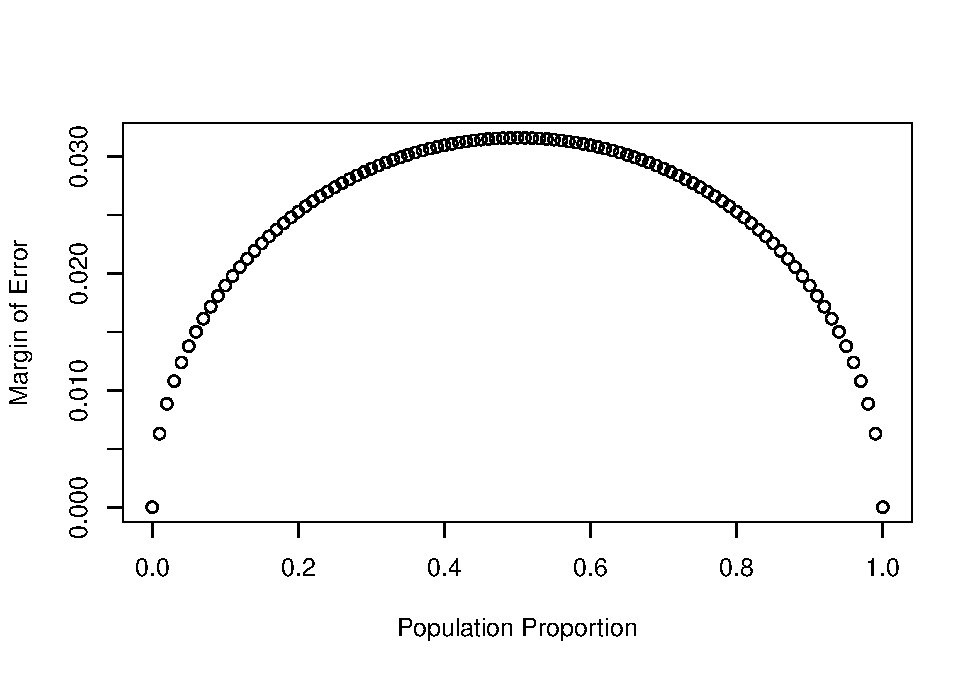
\includegraphics{DATA_606_Lab_6_files/figure-latex/me-plot-1.pdf}

\subsection{Question 8}\label{question-8}

\begin{enumerate}
\def\labelenumi{\arabic{enumi}.}
\setcounter{enumi}{7}
\tightlist
\item
  Describe the relationship between \texttt{p} and \texttt{me}.
\end{enumerate}

\subsubsection{Solution}\label{solution-7}

The margin of error for a sample size is
\(z * \sqrt{\frac{p(1-p)}{n}}\). \(p\) and \(1-p\) are inversely
proportional, which gives us the parabolic effect.

\subsection{Success-failure condition}\label{success-failure-condition}

The textbook emphasizes that you must always check conditions before
making inference. For inference on proportions, the sample proportion
can be assumed to be nearly normal if it is based upon a random sample
of independent observations and if both \(np \geq 10\) and
\(n(1 - p) \geq 10\). This rule of thumb is easy enough to follow, but
it makes one wonder: what's so special about the number 10?

The short answer is: nothing. You could argue that we would be fine with
9 or that we really should be using 11. What is the ``best'' value for
such a rule of thumb is, at least to some degree, arbitrary. However,
when \(np\) and \(n(1-p)\) reaches 10 the sampling distribution is
sufficiently normal to use confidence intervals and hypothesis tests
that are based on that approximation.

We can investigate the interplay between \(n\) and \(p\) and the shape
of the sampling distribution by using simulations. To start off, we
simulate the process of drawing 5000 samples of size 1040 from a
population with a true atheist proportion of 0.1. For each of the 5000
samples we compute \(\hat{p}\) and then plot a histogram to visualize
their distribution.

\begin{Shaded}
\begin{Highlighting}[]
\NormalTok{p <-}\StringTok{ }\FloatTok{0.1}
\NormalTok{n <-}\StringTok{ }\DecValTok{1040}
\NormalTok{p_hats <-}\StringTok{ }\KeywordTok{rep}\NormalTok{(}\DecValTok{0}\NormalTok{, }\DecValTok{5000}\NormalTok{)}

\ControlFlowTok{for}\NormalTok{(i }\ControlFlowTok{in} \DecValTok{1}\OperatorTok{:}\DecValTok{5000}\NormalTok{)\{}
\NormalTok{  samp <-}\StringTok{ }\KeywordTok{sample}\NormalTok{(}\KeywordTok{c}\NormalTok{(}\StringTok{"atheist"}\NormalTok{, }\StringTok{"non_atheist"}\NormalTok{), n, }\DataTypeTok{replace =} \OtherTok{TRUE}\NormalTok{, }\DataTypeTok{prob =} \KeywordTok{c}\NormalTok{(p, }\DecValTok{1}\OperatorTok{-}\NormalTok{p))}
\NormalTok{  p_hats[i] <-}\StringTok{ }\KeywordTok{sum}\NormalTok{(samp }\OperatorTok{==}\StringTok{ "atheist"}\NormalTok{)}\OperatorTok{/}\NormalTok{n}
\NormalTok{\}}

\KeywordTok{hist}\NormalTok{(p_hats, }\DataTypeTok{main =} \StringTok{"p = 0.1, n = 1040"}\NormalTok{, }\DataTypeTok{xlim =} \KeywordTok{c}\NormalTok{(}\DecValTok{0}\NormalTok{, }\FloatTok{0.18}\NormalTok{))}
\end{Highlighting}
\end{Shaded}

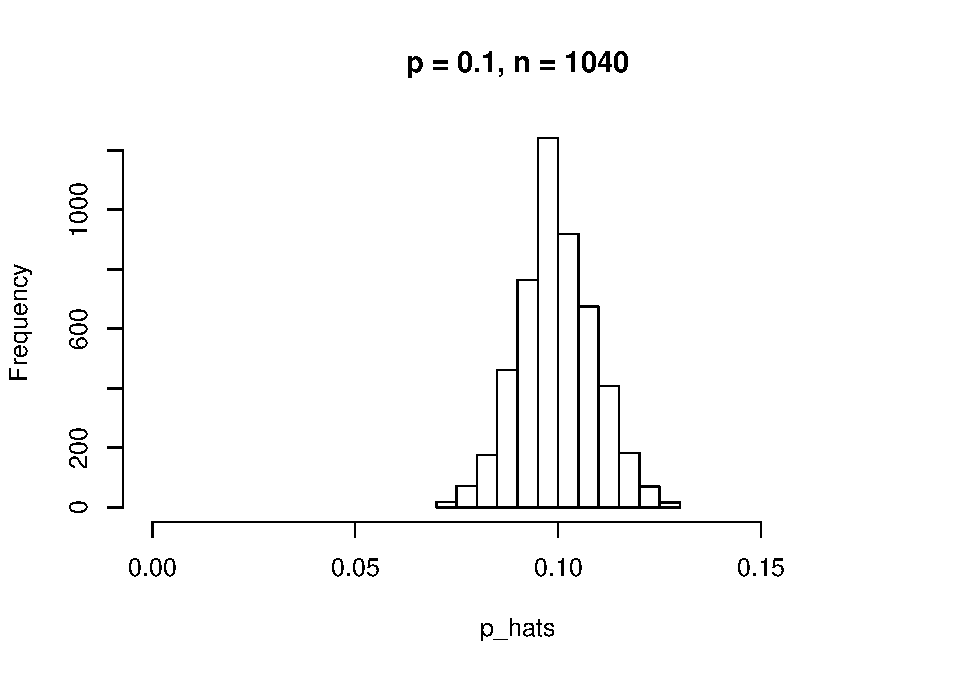
\includegraphics{DATA_606_Lab_6_files/figure-latex/sim-np-1.pdf}

These commands build up the sampling distribution of \(\hat{p}\) using
the familiar \texttt{for} loop. You can read the sampling procedure for
the first line of code inside the \texttt{for} loop as, ``take a sample
of size \(n\) with replacement from the choices of atheist and
non-atheist with probabilities \(p\) and \(1 - p\), respectively.'' The
second line in the loop says, ``calculate the proportion of atheists in
this sample and record this value.'' The loop allows us to repeat this
process 5,000 times to build a good representation of the sampling
distribution.

\subsection{Question 9}\label{question-9}

\begin{enumerate}
\def\labelenumi{\arabic{enumi}.}
\setcounter{enumi}{8}
\tightlist
\item
  Describe the sampling distribution of sample proportions at
  \(n = 1040\) and \(p = 0.1\). Be sure to note the center, spread, and
  shape.\\
  \emph{Hint:} Remember that R has functions such as \texttt{mean} to
  calculate summary statistics.
\end{enumerate}

\subsubsection{Solution}\label{solution-8}

\begin{Shaded}
\begin{Highlighting}[]
\KeywordTok{summary}\NormalTok{(p_hats)}
\end{Highlighting}
\end{Shaded}

\begin{verbatim}
##    Min. 1st Qu.  Median    Mean 3rd Qu.    Max. 
## 0.07019 0.09327 0.09904 0.09969 0.10577 0.12981
\end{verbatim}

From the histogram above, the distribution appears to be normal, with a
center near \texttt{p}.

\subsection{Question 10}\label{question-10}

\begin{enumerate}
\def\labelenumi{\arabic{enumi}.}
\setcounter{enumi}{9}
\tightlist
\item
  Repeat the above simulation three more times but with modified sample
  sizes and proportions: for \(n = 400\) and \(p = 0.1\), \(n = 1040\)
  and \(p = 0.02\), and \(n = 400\) and \(p = 0.02\). Plot all four
  histograms together by running the \texttt{par(mfrow\ =\ c(2,\ 2))}
  command before creating the histograms. You may need to expand the
  plot window to accommodate the larger two-by-two plot. Describe the
  three new sampling distributions. Based on these limited plots, how
  does \(n\) appear to affect the distribution of \(\hat{p}\)? How does
  \(p\) affect the sampling distribution?
\end{enumerate}

\subsubsection{Solution}\label{solution-9}

\begin{Shaded}
\begin{Highlighting}[]
\NormalTok{p <-}\StringTok{ }\FloatTok{0.1}
\NormalTok{n <-}\StringTok{ }\DecValTok{400}
\NormalTok{p_hats1 <-}\StringTok{ }\KeywordTok{rep}\NormalTok{(}\DecValTok{0}\NormalTok{,}\DecValTok{5000}\NormalTok{)}

\ControlFlowTok{for}\NormalTok{(i }\ControlFlowTok{in} \DecValTok{1}\OperatorTok{:}\DecValTok{5000}\NormalTok{)\{}
\NormalTok{  samp <-}\StringTok{ }\KeywordTok{sample}\NormalTok{(}\KeywordTok{c}\NormalTok{(}\StringTok{"atheist"}\NormalTok{, }\StringTok{"non_atheist"}\NormalTok{), n, }\DataTypeTok{replace =} \OtherTok{TRUE}\NormalTok{, }\DataTypeTok{prob =} \KeywordTok{c}\NormalTok{(p, }\DecValTok{1}\OperatorTok{-}\NormalTok{p))}
\NormalTok{  p_hats1[i] <-}\StringTok{ }\KeywordTok{sum}\NormalTok{(samp }\OperatorTok{==}\StringTok{ "atheist"}\NormalTok{)}\OperatorTok{/}\NormalTok{n}
\NormalTok{\}}

\NormalTok{p <-}\StringTok{ }\FloatTok{0.02}
\NormalTok{n <-}\StringTok{ }\DecValTok{1040}
\NormalTok{p_hats2 <-}\StringTok{ }\KeywordTok{rep}\NormalTok{(}\DecValTok{0}\NormalTok{, }\DecValTok{5000}\NormalTok{)}

\ControlFlowTok{for}\NormalTok{(i }\ControlFlowTok{in} \DecValTok{1}\OperatorTok{:}\DecValTok{5000}\NormalTok{)\{}
\NormalTok{  samp <-}\StringTok{ }\KeywordTok{sample}\NormalTok{(}\KeywordTok{c}\NormalTok{(}\StringTok{"atheist"}\NormalTok{, }\StringTok{"non_atheist"}\NormalTok{), n, }\DataTypeTok{replace =} \OtherTok{TRUE}\NormalTok{, }\DataTypeTok{prob =} \KeywordTok{c}\NormalTok{(p, }\DecValTok{1}\OperatorTok{-}\NormalTok{p))}
\NormalTok{  p_hats2[i] <-}\StringTok{ }\KeywordTok{sum}\NormalTok{(samp }\OperatorTok{==}\StringTok{ "atheist"}\NormalTok{)}\OperatorTok{/}\NormalTok{n}
\NormalTok{\}}


\NormalTok{p <-}\StringTok{ }\FloatTok{0.02}
\NormalTok{n <-}\StringTok{ }\DecValTok{400}
\NormalTok{p_hats3 <-}\StringTok{ }\KeywordTok{rep}\NormalTok{(}\DecValTok{0}\NormalTok{, }\DecValTok{5000}\NormalTok{)}

\ControlFlowTok{for}\NormalTok{(i }\ControlFlowTok{in} \DecValTok{1}\OperatorTok{:}\DecValTok{5000}\NormalTok{)\{}
\NormalTok{  samp <-}\StringTok{ }\KeywordTok{sample}\NormalTok{(}\KeywordTok{c}\NormalTok{(}\StringTok{"atheist"}\NormalTok{, }\StringTok{"non_atheist"}\NormalTok{), n, }\DataTypeTok{replace =} \OtherTok{TRUE}\NormalTok{, }\DataTypeTok{prob =} \KeywordTok{c}\NormalTok{(p, }\DecValTok{1}\OperatorTok{-}\NormalTok{p))}
\NormalTok{  p_hats3[i] <-}\StringTok{ }\KeywordTok{sum}\NormalTok{(samp }\OperatorTok{==}\StringTok{ "atheist"}\NormalTok{)}\OperatorTok{/}\NormalTok{n}
\NormalTok{\}}


\KeywordTok{par}\NormalTok{(}\DataTypeTok{mfrow =} \KeywordTok{c}\NormalTok{(}\DecValTok{2}\NormalTok{, }\DecValTok{2}\NormalTok{))}
\KeywordTok{hist}\NormalTok{(p_hats, }\DataTypeTok{main =} \StringTok{"p = 0.1, n = 1040"}\NormalTok{)}
\KeywordTok{hist}\NormalTok{(p_hats1, }\DataTypeTok{main =} \StringTok{"p = 0.1, n = 400"}\NormalTok{)}
\KeywordTok{hist}\NormalTok{(p_hats2, }\DataTypeTok{main =} \StringTok{"p = 0.02, n = 1040"}\NormalTok{)}
\KeywordTok{hist}\NormalTok{(p_hats3, }\DataTypeTok{main =} \StringTok{"p = 0.02, n = 400"}\NormalTok{)}
\end{Highlighting}
\end{Shaded}

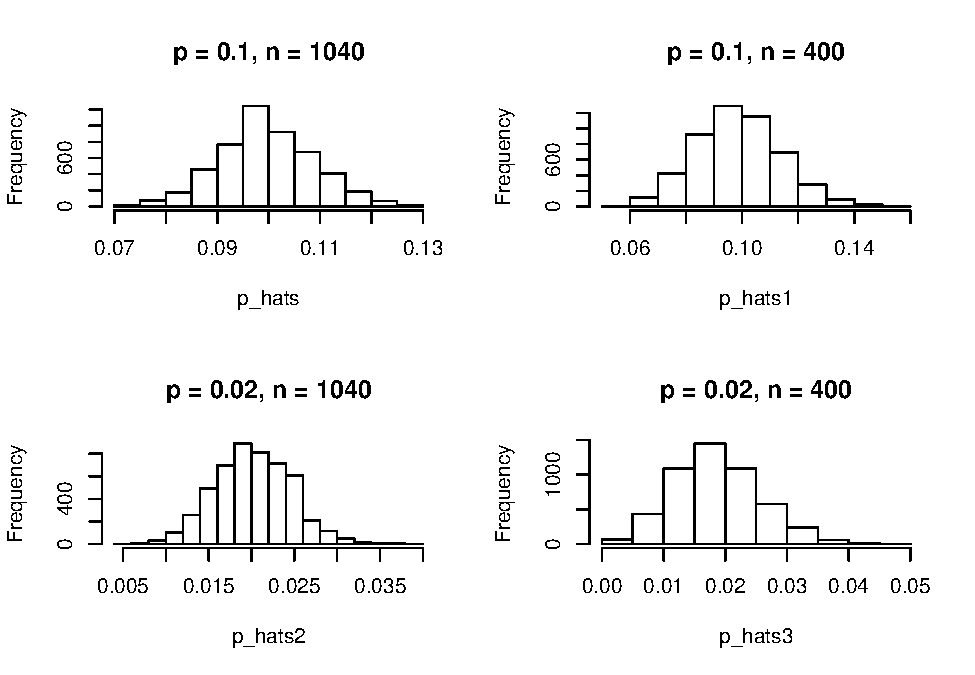
\includegraphics{DATA_606_Lab_6_files/figure-latex/unnamed-chunk-5-1.pdf}

Once you're done, you can reset the layout of the plotting window by
using the command \texttt{par(mfrow\ =\ c(1,\ 1))} command or clicking
on ``Clear All'' above the plotting window (if using RStudio). Note that
the latter will get rid of all your previous plots.

\subsection{Question 6}\label{question-6-1}

\begin{enumerate}
\def\labelenumi{\arabic{enumi}.}
\setcounter{enumi}{10}
\tightlist
\item
  If you refer to Table 6, you'll find that Australia has a sample
  proportion of 0.1 on a sample size of 1040, and that Ecuador has a
  sample proportion of 0.02 on 400 subjects. Let's suppose for this
  exercise that these point estimates are actually the truth. Then given
  the shape of their respective sampling distributions, do you think it
  is sensible to proceed with inference and report margin of errors, as
  the reports does?
\end{enumerate}

\subsubsection{Solution}\label{solution-10}

The only issue is with Ecuador. Since \(0.02 \times 400 = 8\), it
doesn't pass the success-failure condition.

\begin{center}\rule{0.5\linewidth}{\linethickness}\end{center}

\subsection{On your own}\label{on-your-own}

The question of atheism was asked by WIN-Gallup International in a
similar survey that was conducted in 2005. (We assume here that sample
sizes have remained the same.) Table 4 on page 13 of the report
summarizes survey results from 2005 and 2012 for 39 countries.

\subsection{Question 12}\label{question-12}

Answer the following two questions using the \texttt{inference}
function. As always, write out the hypotheses for any tests you conduct
and outline the status of the conditions for inference.

\subsubsection{Part a}\label{part-a}

\textbf{a.} Is there convincing evidence that Spain has seen a change in
its atheism index between 2005 and 2012?~\emph{Hint:} Create a new data
set for respondents from Spain. Form confidence intervals for the true
proportion of athiests in both years, and determine whether they
overlap.

\paragraph{Solution}\label{solution-11}

\(H_0:\) The proportion of atheists in Spain is the same in 2012 as it
was in 2005. \(H_A\): The proportion differs.

\begin{Shaded}
\begin{Highlighting}[]
\NormalTok{es05 <-}\StringTok{ }\KeywordTok{subset}\NormalTok{(atheism, nationality }\OperatorTok{==}\StringTok{ "Spain"} \OperatorTok{&}\StringTok{ }\NormalTok{year }\OperatorTok{==}\StringTok{ "2005"}\NormalTok{)}
\NormalTok{es12 <-}\StringTok{ }\KeywordTok{subset}\NormalTok{(atheism, nationality }\OperatorTok{==}\StringTok{ "Spain"} \OperatorTok{&}\StringTok{ }\NormalTok{year }\OperatorTok{==}\StringTok{ "2012"}\NormalTok{)}

\KeywordTok{sum}\NormalTok{(es05}\OperatorTok{$}\NormalTok{response }\OperatorTok{==}\StringTok{ "atheist"}\NormalTok{) }\OperatorTok{/}\StringTok{ }\KeywordTok{nrow}\NormalTok{(es05)}
\end{Highlighting}
\end{Shaded}

\begin{verbatim}
## [1] 0.100349
\end{verbatim}

\begin{Shaded}
\begin{Highlighting}[]
\KeywordTok{sum}\NormalTok{(es12}\OperatorTok{$}\NormalTok{response }\OperatorTok{==}\StringTok{ "atheist"}\NormalTok{) }\OperatorTok{/}\StringTok{ }\KeywordTok{nrow}\NormalTok{(es12)}
\end{Highlighting}
\end{Shaded}

\begin{verbatim}
## [1] 0.08995633
\end{verbatim}

\begin{Shaded}
\begin{Highlighting}[]
\KeywordTok{inference}\NormalTok{(es05}\OperatorTok{$}\NormalTok{response, }\DataTypeTok{est =} \StringTok{"proportion"}\NormalTok{, }\DataTypeTok{type =} \StringTok{"ci"}\NormalTok{, }\DataTypeTok{method =} \StringTok{"theoretical"}\NormalTok{, }\DataTypeTok{success =} \StringTok{"atheist"}\NormalTok{)}
\end{Highlighting}
\end{Shaded}

\begin{verbatim}
## Single proportion -- success: atheist 
## Summary statistics:
\end{verbatim}

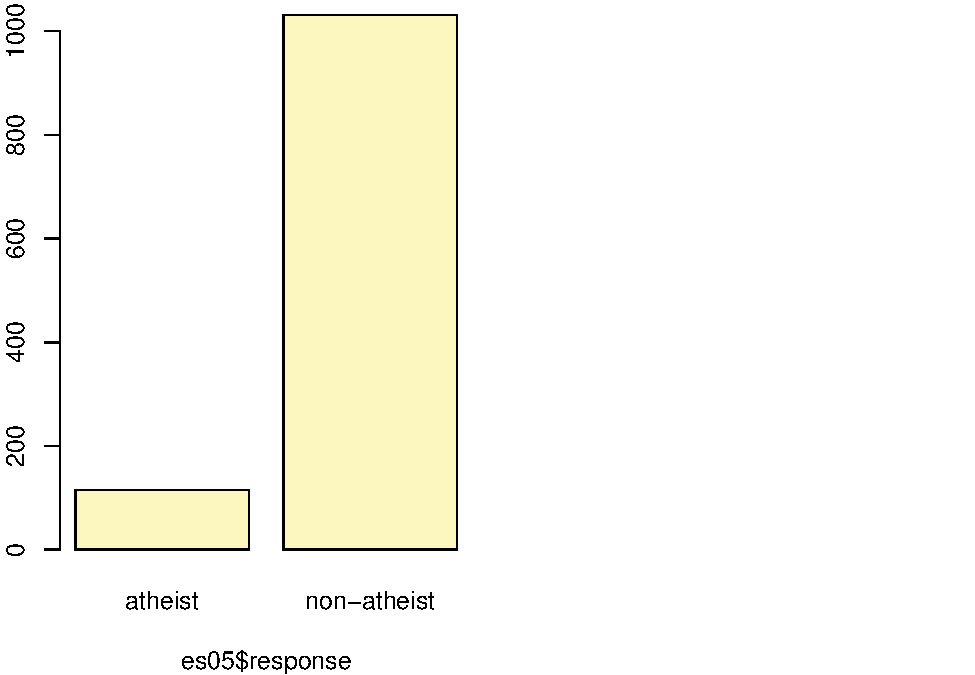
\includegraphics{DATA_606_Lab_6_files/figure-latex/unnamed-chunk-6-1.pdf}

\begin{verbatim}
## p_hat = 0.1003 ;  n = 1146 
## Check conditions: number of successes = 115 ; number of failures = 1031 
## Standard error = 0.0089 
## 95 % Confidence interval = ( 0.083 , 0.1177 )
\end{verbatim}

\begin{Shaded}
\begin{Highlighting}[]
\KeywordTok{inference}\NormalTok{(es12}\OperatorTok{$}\NormalTok{response, }\DataTypeTok{est =} \StringTok{"proportion"}\NormalTok{, }\DataTypeTok{type =} \StringTok{"ci"}\NormalTok{, }\DataTypeTok{method =} \StringTok{"theoretical"}\NormalTok{, }\DataTypeTok{success =} \StringTok{"atheist"}\NormalTok{)}
\end{Highlighting}
\end{Shaded}

\begin{verbatim}
## Single proportion -- success: atheist 
## Summary statistics:
\end{verbatim}

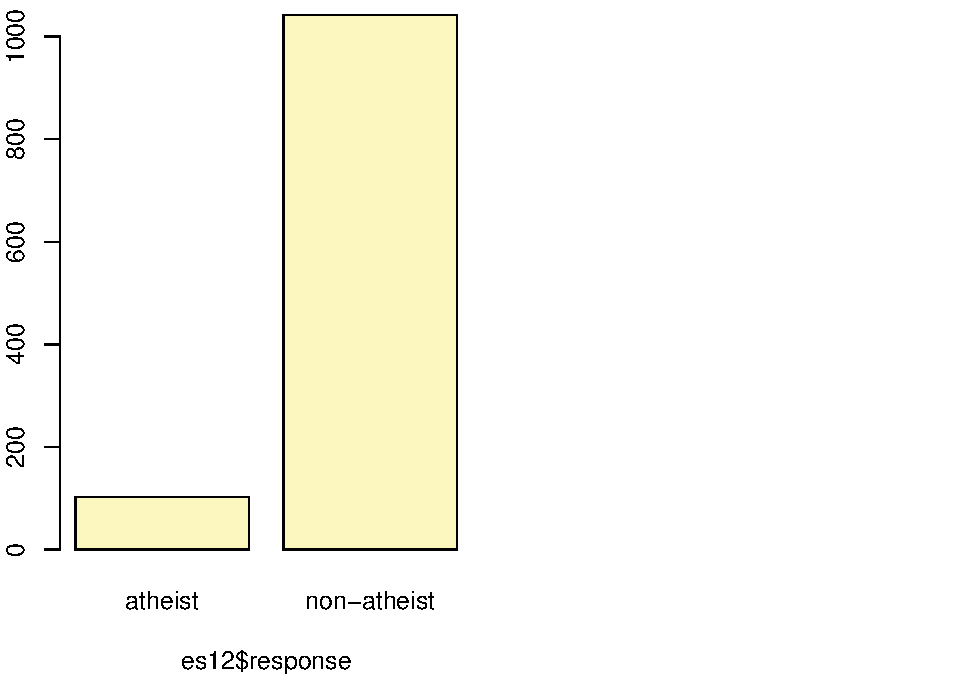
\includegraphics{DATA_606_Lab_6_files/figure-latex/unnamed-chunk-6-2.pdf}

\begin{verbatim}
## p_hat = 0.09 ;  n = 1145 
## Check conditions: number of successes = 103 ; number of failures = 1042 
## Standard error = 0.0085 
## 95 % Confidence interval = ( 0.0734 , 0.1065 )
\end{verbatim}

First, we note that all conditions for inference are satisfied. Since
the p-value = \(0.3966 > 0.05\), and the confidence intervals overlap,
we don't have enough evidence to reject the null hypothesis, and
conclude that the proportion of atheists in Spain is the same in 2005
and 2012.

\subsubsection{Part b}\label{part-b}

\textbf{b.} Is there convincing evidence that the United States has seen
a change in its atheism index between 2005 and 2012?

\paragraph{Solution}\label{solution-12}

\begin{Shaded}
\begin{Highlighting}[]
\CommentTok{# us12 was calculated earlier}
\NormalTok{us05 <-}\StringTok{ }\KeywordTok{subset}\NormalTok{(atheism, nationality }\OperatorTok{==}\StringTok{ "United States"} \OperatorTok{&}\StringTok{ }\NormalTok{year }\OperatorTok{==}\StringTok{ "2005"}\NormalTok{)}

\KeywordTok{sum}\NormalTok{(us05}\OperatorTok{$}\NormalTok{response}\OperatorTok{==}\StringTok{"atheist"}\NormalTok{) }\OperatorTok{/}\StringTok{ }\KeywordTok{nrow}\NormalTok{(us05)}
\end{Highlighting}
\end{Shaded}

\begin{verbatim}
## [1] 0.00998004
\end{verbatim}

\begin{Shaded}
\begin{Highlighting}[]
\KeywordTok{sum}\NormalTok{(us12}\OperatorTok{$}\NormalTok{response}\OperatorTok{==}\StringTok{"atheist"}\NormalTok{) }\OperatorTok{/}\StringTok{ }\KeywordTok{nrow}\NormalTok{(us12)}
\end{Highlighting}
\end{Shaded}

\begin{verbatim}
## [1] 0.1394892
\end{verbatim}

\begin{Shaded}
\begin{Highlighting}[]
\KeywordTok{inference}\NormalTok{(us05}\OperatorTok{$}\NormalTok{response, }\DataTypeTok{est =} \StringTok{"proportion"}\NormalTok{, }\DataTypeTok{type =} \StringTok{"ci"}\NormalTok{, }\DataTypeTok{method =} \StringTok{"theoretical"}\NormalTok{, }\DataTypeTok{success =} \StringTok{"atheist"}\NormalTok{)}
\end{Highlighting}
\end{Shaded}

\begin{verbatim}
## Single proportion -- success: atheist 
## Summary statistics:
\end{verbatim}

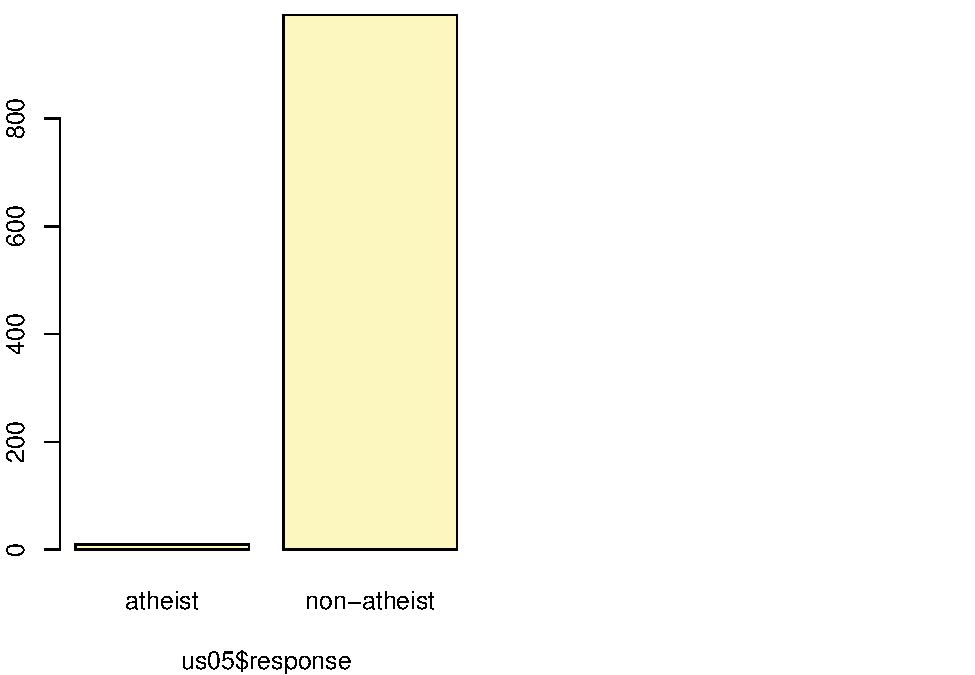
\includegraphics{DATA_606_Lab_6_files/figure-latex/unnamed-chunk-7-1.pdf}

\begin{verbatim}
## p_hat = 0.01 ;  n = 1002 
## Check conditions: number of successes = 10 ; number of failures = 992 
## Standard error = 0.0031 
## 95 % Confidence interval = ( 0.0038 , 0.0161 )
\end{verbatim}

\begin{Shaded}
\begin{Highlighting}[]
\KeywordTok{inference}\NormalTok{(us12}\OperatorTok{$}\NormalTok{response, }\DataTypeTok{est =} \StringTok{"proportion"}\NormalTok{, }\DataTypeTok{type =} \StringTok{"ci"}\NormalTok{, }\DataTypeTok{method =} \StringTok{"theoretical"}\NormalTok{, }\DataTypeTok{success =} \StringTok{"atheist"}\NormalTok{)}
\end{Highlighting}
\end{Shaded}

\begin{verbatim}
## Single proportion -- success: atheist 
## Summary statistics:
\end{verbatim}

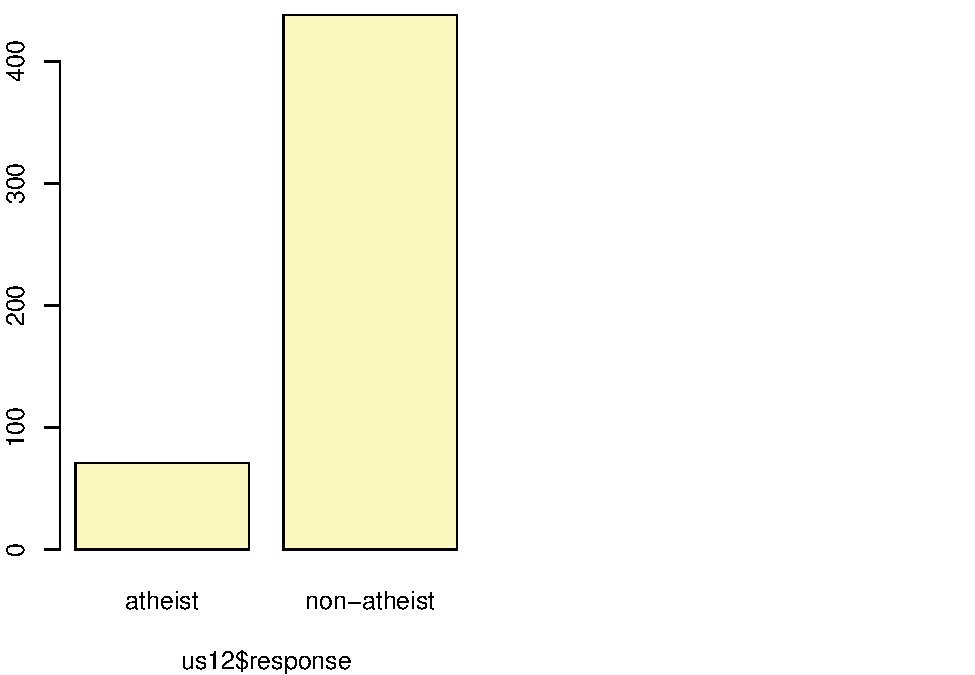
\includegraphics{DATA_606_Lab_6_files/figure-latex/unnamed-chunk-7-2.pdf}

\begin{verbatim}
## p_hat = 0.1395 ;  n = 509 
## Check conditions: number of successes = 71 ; number of failures = 438 
## Standard error = 0.0154 
## 95 % Confidence interval = ( 0.1094 , 0.1696 )
\end{verbatim}

First, we note that all the conditions for inference are satisfied.
Since the p-value is \(\approx 0\), and the confidence intervals do not
overlap, we can reject the null hypothesis, and conclude that the
proportion of atheists in the US differs in the years 2005 and 2012.

\subsection{Question 12}\label{question-12-1}

If in fact there has been no change in the atheism index in the
countries listed in Table 4, in how many of those countries would you
expect to detect a change (at a significance level of 0.05) simply by
chance?\\
\emph{Hint:} Look in the textbook index under Type 1 error.

\subsubsection{Solution}\label{solution-13}

A Type 1 error occurs when we wrongly reject the null hypothesis. At a
significance level of 0.05, we do not want it to occur more than \(5\%\)
of the time. Since there are 39 countries, we'd expect to see change in
approximately \(39 \times 0.05 \approx 2\) countries.

\subsection{Question 13}\label{question-13}

Suppose you're hired by the local government to estimate the proportion
of residents that attend a religious service on a weekly basis.
According to the guidelines, the estimate must have a margin of error no
greater than 1\% with 95\% confidence. You have no idea what to expect
for \(p\). How many people would you have to sample to ensure that you
are within the guidelines?\\
\emph{Hint:} Refer to your plot of the relationship between \(p\) and
margin of error. Do not use the data set to answer this question.

\subsubsection{Solution}\label{solution-14}

We assume that the margin of error is highest at \(p = 0.5\). Plugging
this into our formula, and solving for \(n\) :\\
\(ME = z * SE\)\\
\(SE = \sqrt{\frac{p\cdot(1-p)}{n}}\)\\
\(\frac{ME}{z} = \sqrt{\frac{p\cdot(1-p)}{n}} \to \Big(\frac{ME}{z}\Big)^2 = \frac{p\cdot(1-p)}{n}\)\\
Plugging in our values, we get:\\
\(n \geq (1.96)^2\times\frac{0.5(1-0.5)}{(0.01)^2}\)\\
Solving for \(n\), we need at least \(9604\) people to ensure a margin
of error \(\leq 1\%\) with \(95\%\) confidence.


\end{document}
